\documentclass[tikz,border=2pt]{standalone}
\usepackage{amsmath,amssymb}
\usepackage{pgfplots}
\pgfplotsset{compat=1.18}

\begin{document}
% Hypergeometric pmf: draw n = 6 objects without replacement from N = 20 of which K = 8 are
% successes; X counts the successes drawn. Mean n K / N = 2.4.
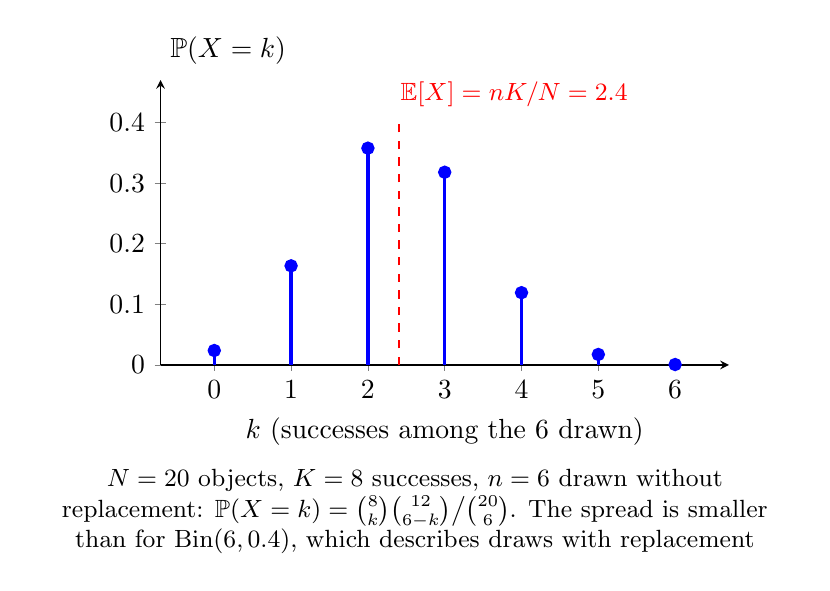
\begin{tikzpicture}
	\begin{axis}[
		axis lines=left, xmin=-0.7, xmax=6.7, ymin=0, ymax=0.47,
		xtick={0,...,6}, ytick={0,0.1,0.2,0.3,0.4},
		xlabel={$k$ (successes among the $6$ drawn)}, ylabel={$\mathbb{P}(X=k)$}, ylabel style={rotate=-90, anchor=south west, at={(axis description cs:0,1.02)}},
		width=8.8cm, height=5.2cm, clip=false
		]
		\addplot[ycomb, blue, very thick, mark=*, mark size=1.8pt] coordinates {(0,0.0238) (1,0.1635) (2,0.3576) (3,0.3179) (4,0.1192) (5,0.0173) (6,0.0007)};
		\draw[red, dashed, thick] (axis cs:2.4,0) -- (axis cs:2.4,0.41);
		\node[red, anchor=south west, font=\small] at (axis cs:2.3,0.41) {$\mathbb{E}[X]=nK/N=2.4$};
	\end{axis}
	\node[anchor=north, font=\small, align=flush center, text width=9.6cm] at ([yshift=-2pt]current axis.outer south) {$N=20$ objects, $K=8$ successes, $n=6$ drawn without replacement: $\mathbb{P}(X=k)=\binom8k\binom{12}{6-k}\big/\binom{20}6$. The spread is smaller than for $\operatorname{Bin}(6,0.4)$, which describes draws with replacement};
\end{tikzpicture}
\end{document}
